\section{RNN Encoder--Decoder}
\label{sec:detail}

In this document, we describe in detail the architecture of the RNN
Encoder--Decoder used in the experiments.

Let us denote an source phrase by $X=\left( \vx_1, \vx_2, \dots, \vx_N \right)$
and a target phrase by $Y=\left( \vy_1, \vy_2, \dots, \vy_M \right)$. Each
phrase is a sequence of $K$-dimensional one-hot vectors, such that only one
element of the vector is $1$ and all the others are $0$. The index of the active
($1$) element indicates the word represented by the vector.

\subsection{Encoder}

Each word of the source phrase is embedded in a $500$-dimensional vector space:
$e(\vx_i) \in \RR^{500}$. $e(\vx)$ is used in Sec.~\ref{sec:rep} to visualize
the words.

The hidden state of an encoder consists of $1000$ hidden units,
and each one of them at time $t$ is computed by
\begin{align*}
    h_j^{\qt{t}} = z_j h_j^{\qt{t-1}} + (1 - z_j) \tilde{h}_j^{\qt{t}},
\end{align*}
where
\begin{align*}
    \tilde{h}_j^{\qt{t}} =& \tanh\left( \left[ \mW e(\vx_t) \right]_j + \left[
    \mU \left( \vr \odot \vh_{\qt{t-1}}\right) \right]_j \right),
    \\
    z_j =& \sigma\left( \left[ \mW_z e(\vx_t) \right]_j + 
    \left[\mU_z \vh_{\qt{t-1}}\right]_j \right),
    \\
    r_j =& \sigma\left( \left[ \mW_r e(\vx_t) \right]_j + 
    \left[\mU_r \vh_{\qt{t-1}}\right]_j \right).
\end{align*}
$\sigma$ and $\odot$ are a logistic sigmoid function and an element-wise
multiplication, respectively. To make the equations uncluttered, we omit
biases. The initial hidden state $h_j^{\qt{0}}$ is fixed to $0$.

Once the hidden state at the $N$ step (the end of the source
phrase) is computed, the representation of the source phrase
$\vc$ is
\begin{align*}
    \vc = \tanh \left( \mV \vh^{\qt{N}} \right).
\end{align*}

\subsubsection{Decoder}

The decoder starts by initializing the hidden state with
\begin{align*}
    {\vh'}^{\qt{0}} = \tanh \left( \mV' \vc \right),
\end{align*}
where we will use $\cdot'$ to distinguish parameters of the
decoder from those of the encoder.

The hidden state at time $t$ of the decoder is computed by
\begin{align*}
    {h'}_j^{\qt{t}} = {z'}_j {h'}_j^{\qt{t-1}} +
    (1 - {z'}_j) \tilde{h'}_j^{\qt{t}},
\end{align*}
where
\begin{align*}
    \tilde{h'}_j^{\qt{t}} =& \tanh\left( 
    \left[ \mW' e(\vy_{t-1}) \right]_j + 
    {r'}_j \left[ \mU' {\vh'}_{\qt{t-1}} +
    \mC \vc 
    \right]
    \right),
    \\
    {z'}_j =& \sigma\left( \left[ {\mW'}_z e(\vy_{t-1}) \right]_j + 
    \left[{\mU'}_z {\vh'}_{\qt{t-1}}\right]_j +
    \left[\mC_z \vc \right]_j 
    \right),
    \\
    {r'}_j =& \sigma\left( \left[ {\mW'}_r e(\vy_{t-1}) \right]_j + 
    \left[{\mU'}_r {\vh'}_{\qt{t-1}}\right]_j +
    \left[ \mC_r \vc \right]_j
    \right),
\end{align*}
and $e(\vy_{0})$ is an all-zero vector. Similarly to the case of
the encoder, $e(\vy)$ is an embedding of a target word.

Unlike the encoder which simply encodes the source phrase, the
decoder is learned to generate a target phrase. At each time $t$,
the decoder computes the probability of generating $j$-th word by
\begin{align*}
    p(y_{t,j} = 1 \mid \vy_{t-1}, \dots, \vy_1, X) = \frac{\exp
        \left( {\vg}_j \vs_{\qt{t}}\right) } {\sum_{j'=1}^{K}
        \exp \left( \vg_{j'} \vs_{\qt{t}}\right) },
\end{align*}
where the $i$-element of $\vs_{\qt{t}}$ is 
\begin{align*}
    s_i^{\qt{t}} = \max\left\{
    {s'}_{2i-1}^{\qt{t}}, {s'}_{2i}^{\qt{t}}
\right\}
\end{align*}
and
\begin{align*}
    {\vs'}^{\qt{t}} = \mO_h {\vh'}^{\qt{t}} + \mO_y \vy_{t-1} + \mO_c \vc.
\end{align*}
In short, the $s_i^{\qt{t}}$ is a so-called \textit{maxout} unit.

For the computational efficiency, instead of a single-matrix
output weight $\mG$, we use a product of two matrices such that
\begin{align*}
    \mG = \mG_l \mG_r,
\end{align*}
where $\mG_l \in \RR^{K \times 500}$ and $\mG_r \in \RR^{500 \times
1000}$.


\section{Word and Phrase Representations}
\label{sec:word_phrase_embed}

Here, we show enlarged plots of the word and phrase
representations in
Figs.~\ref{fig:word_embed}--\ref{fig:phrase_embed}.

\newpage
\begin{landscape}
\begin{figure*}[p]
    \iftoggle{arxiv}{
        \vspace{-20mm}
    }
    \centering
    \begin{minipage}{0.75\textwidth}
        \centering
        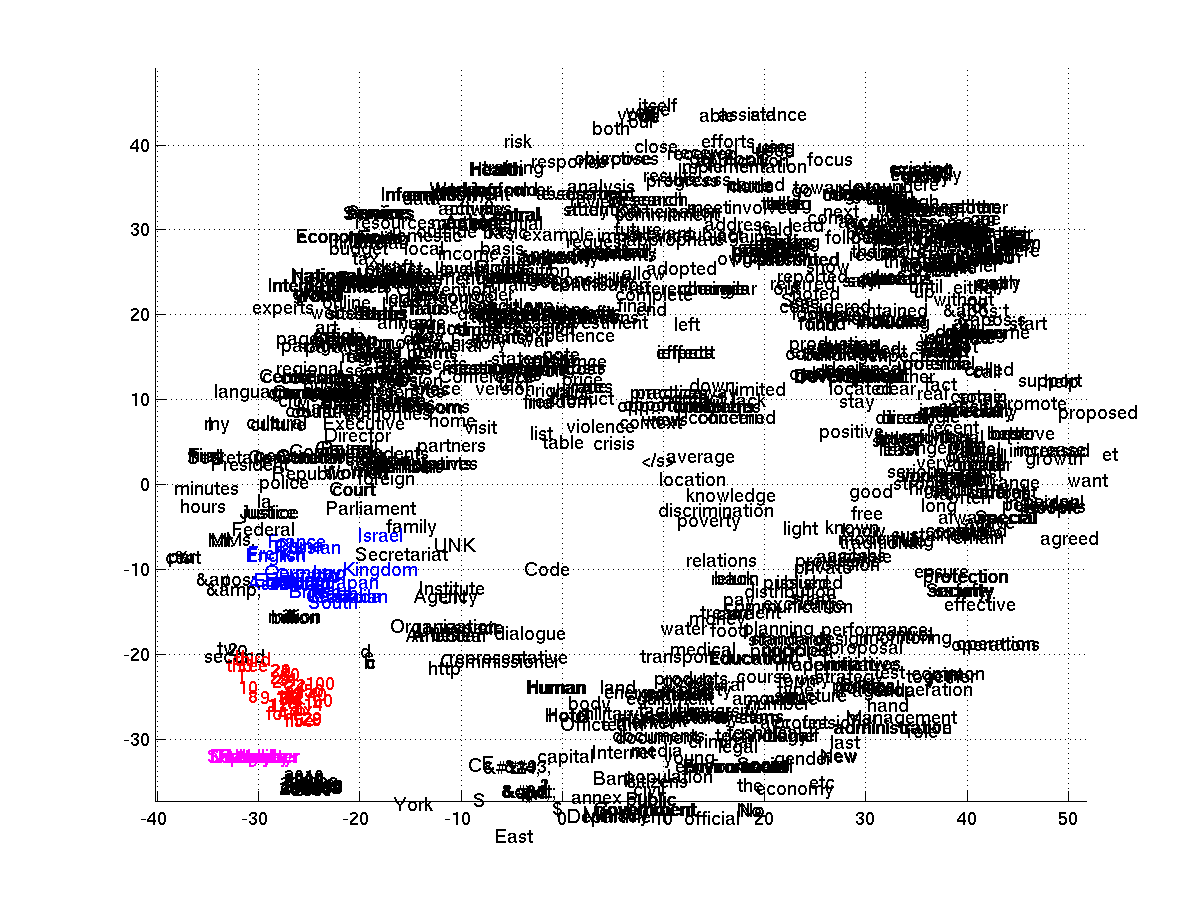
\includegraphics[width=0.99\textwidth]{word_all.png}
    \end{minipage}
    \begin{minipage}{0.75\textwidth}
        \centering
        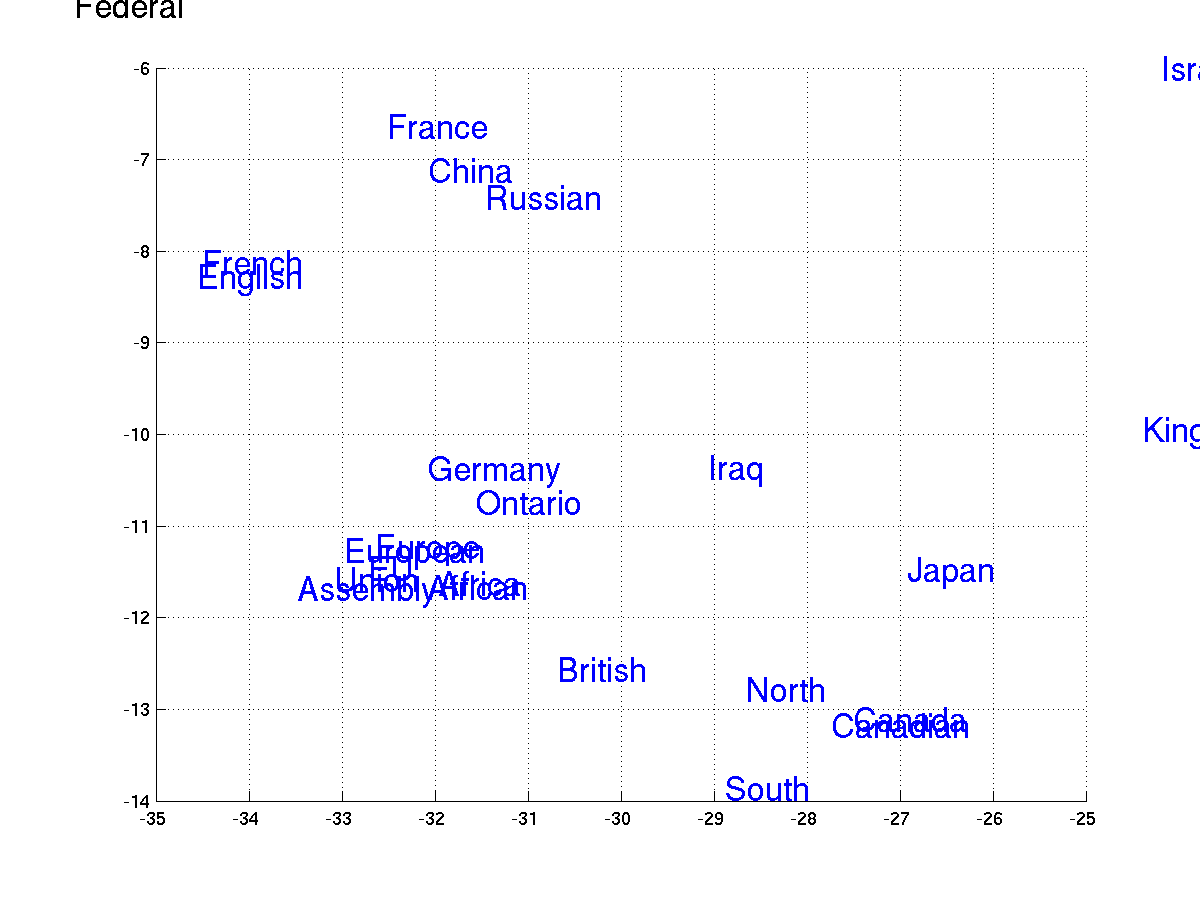
\includegraphics[width=0.99\textwidth]{word_countries.png}
    \end{minipage}
    \\
    \begin{minipage}{0.75\textwidth}
        \centering
        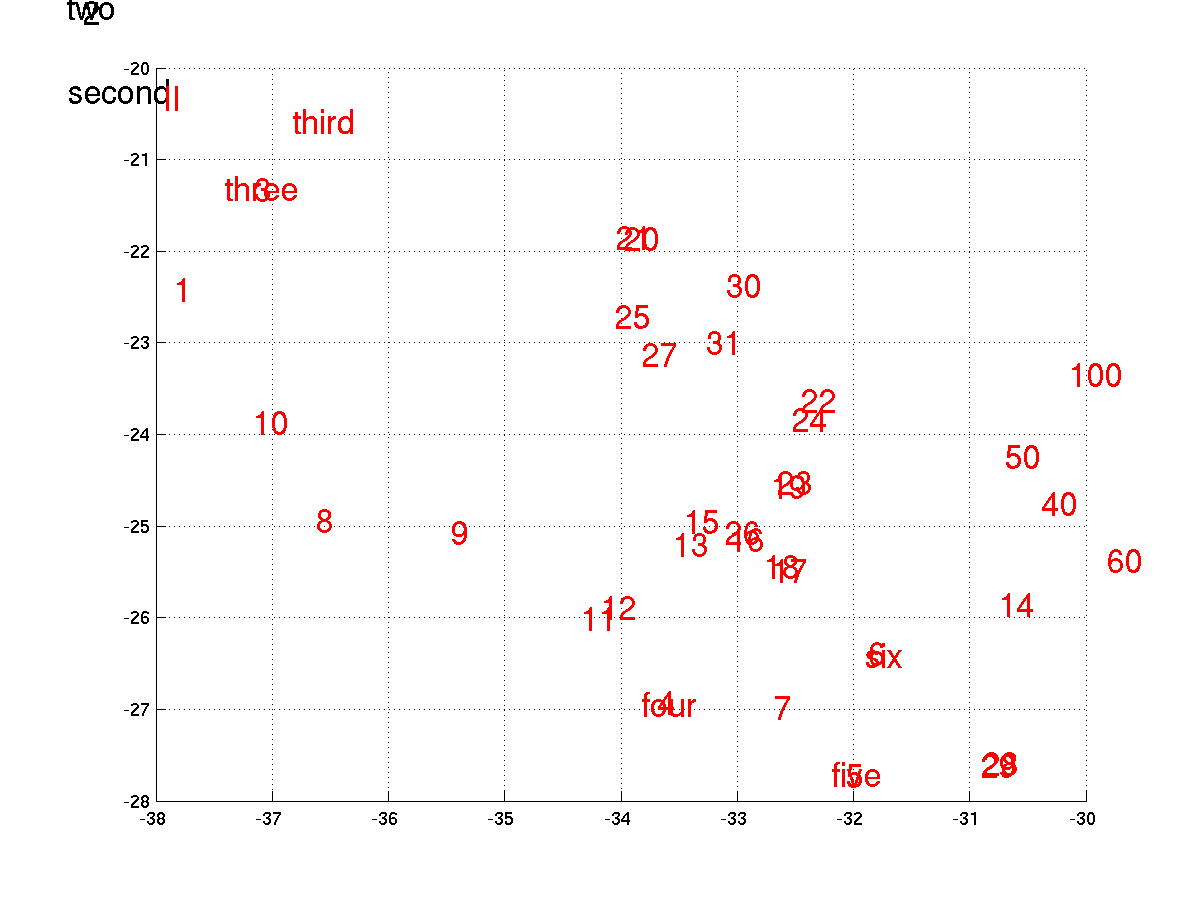
\includegraphics[width=0.99\textwidth]{word_numbers.png}
    \end{minipage}
    \begin{minipage}{0.75\textwidth}
        \centering
        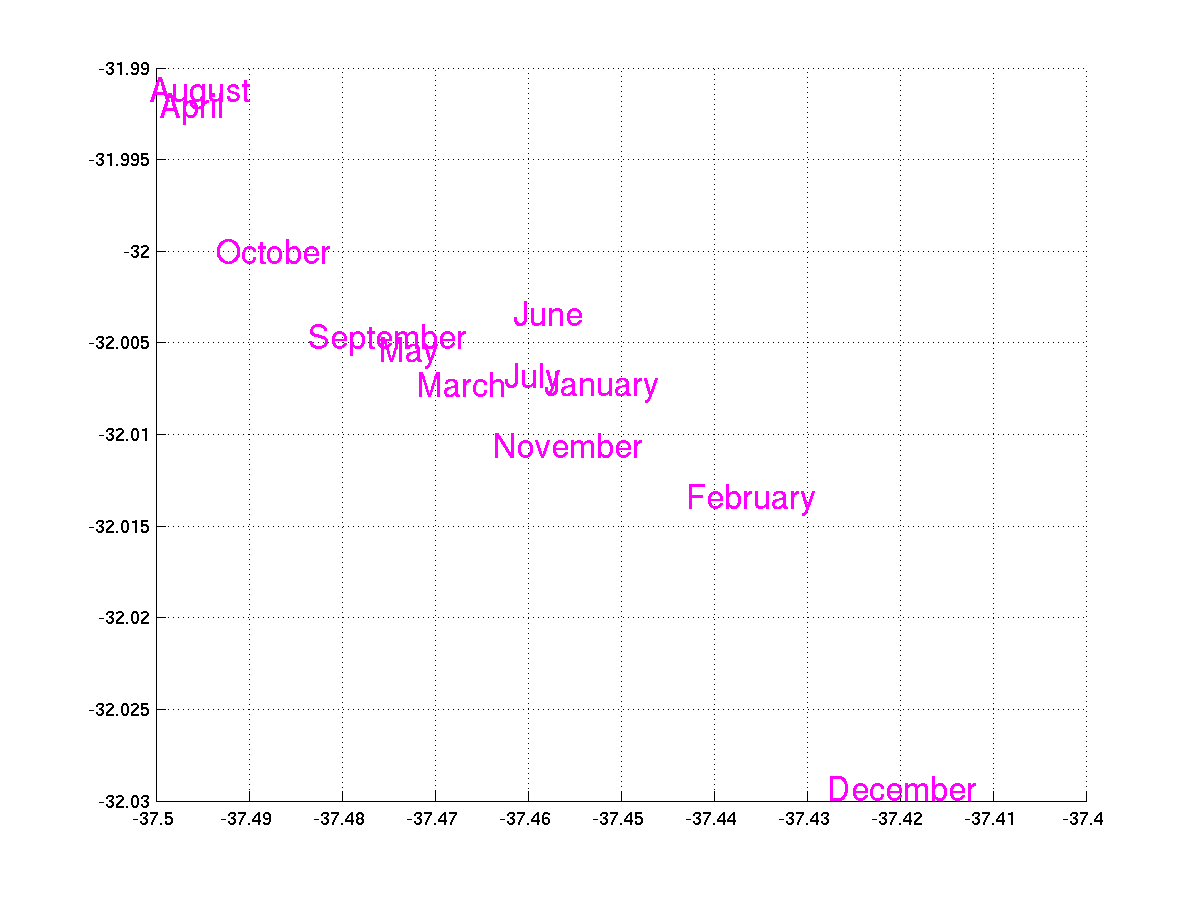
\includegraphics[width=0.99\textwidth]{word_months.png}
    \end{minipage}
    \caption{2--D embedding of the learned word representation. The top left one
        shows the full embedding space, while the other three figures show the
    zoomed-in view of specific regions (color--coded).} 
\end{figure*}
\end{landscape}


\newpage
\begin{landscape}
\begin{figure*}[p]
    \iftoggle{arxiv}{
        \vspace{-20mm}
    }
    \centering
    \begin{minipage}{0.75\textwidth}
        \centering
        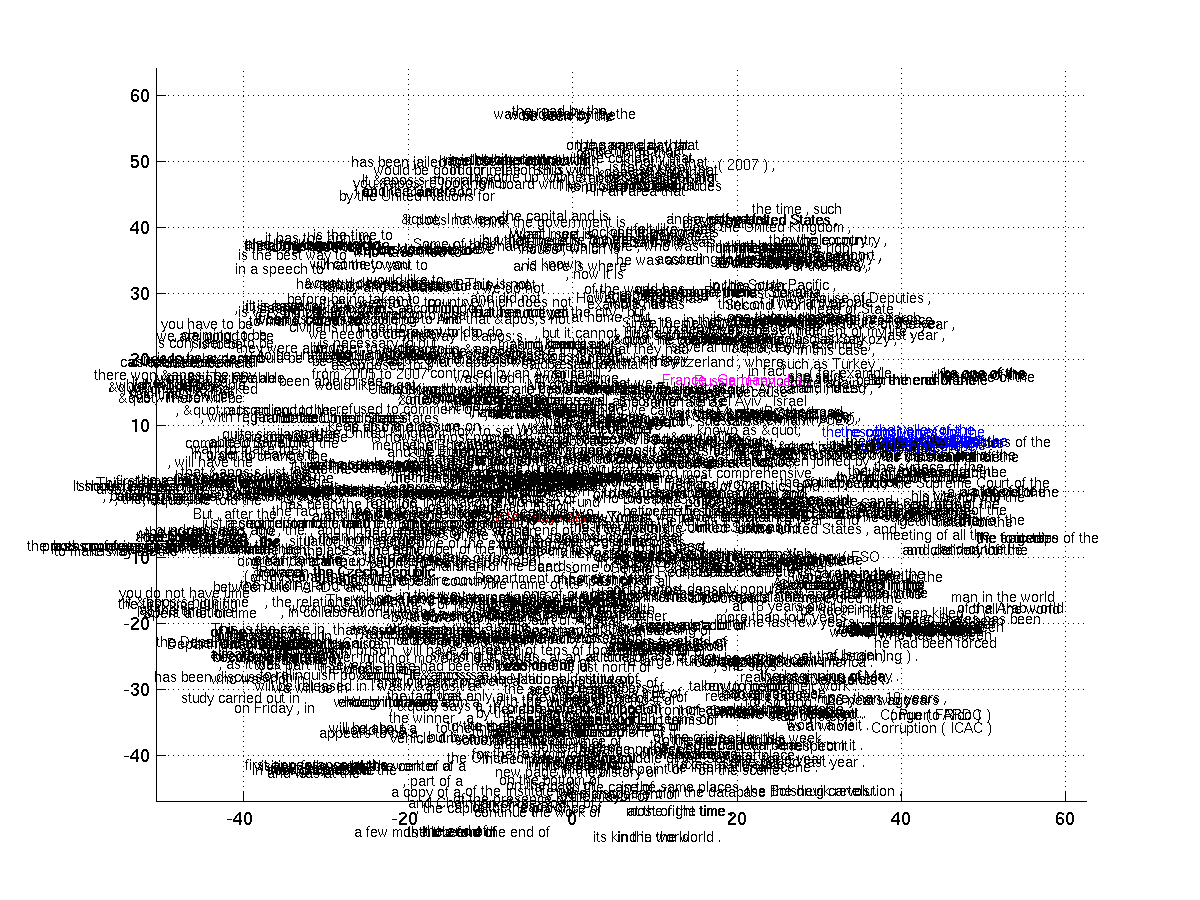
\includegraphics[width=0.99\textwidth]{phrase_all.png}
    \end{minipage}
    \begin{minipage}{0.75\textwidth}
        \centering
        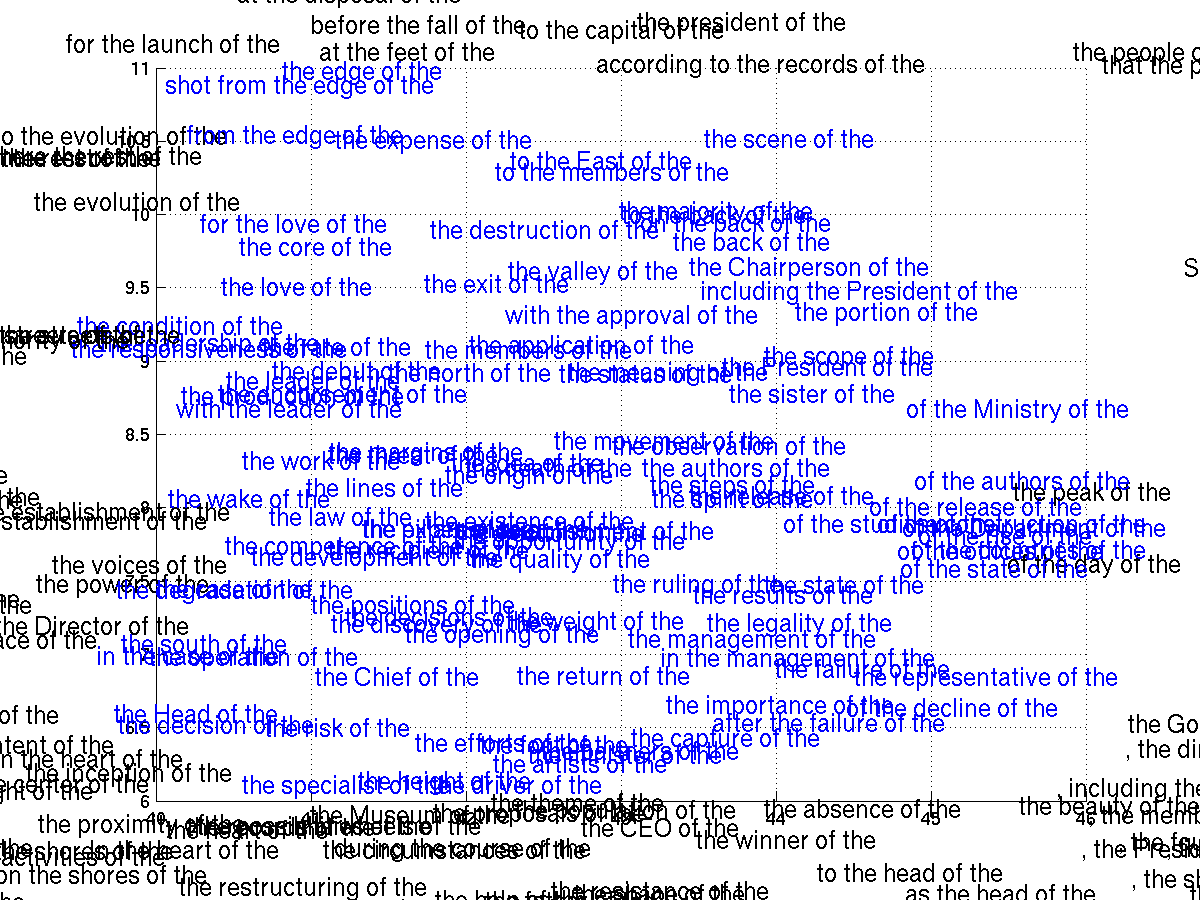
\includegraphics[width=0.99\textwidth]{phrase_zoom1.png}
    \end{minipage}
    \\
    \begin{minipage}{0.75\textwidth}
        \centering
        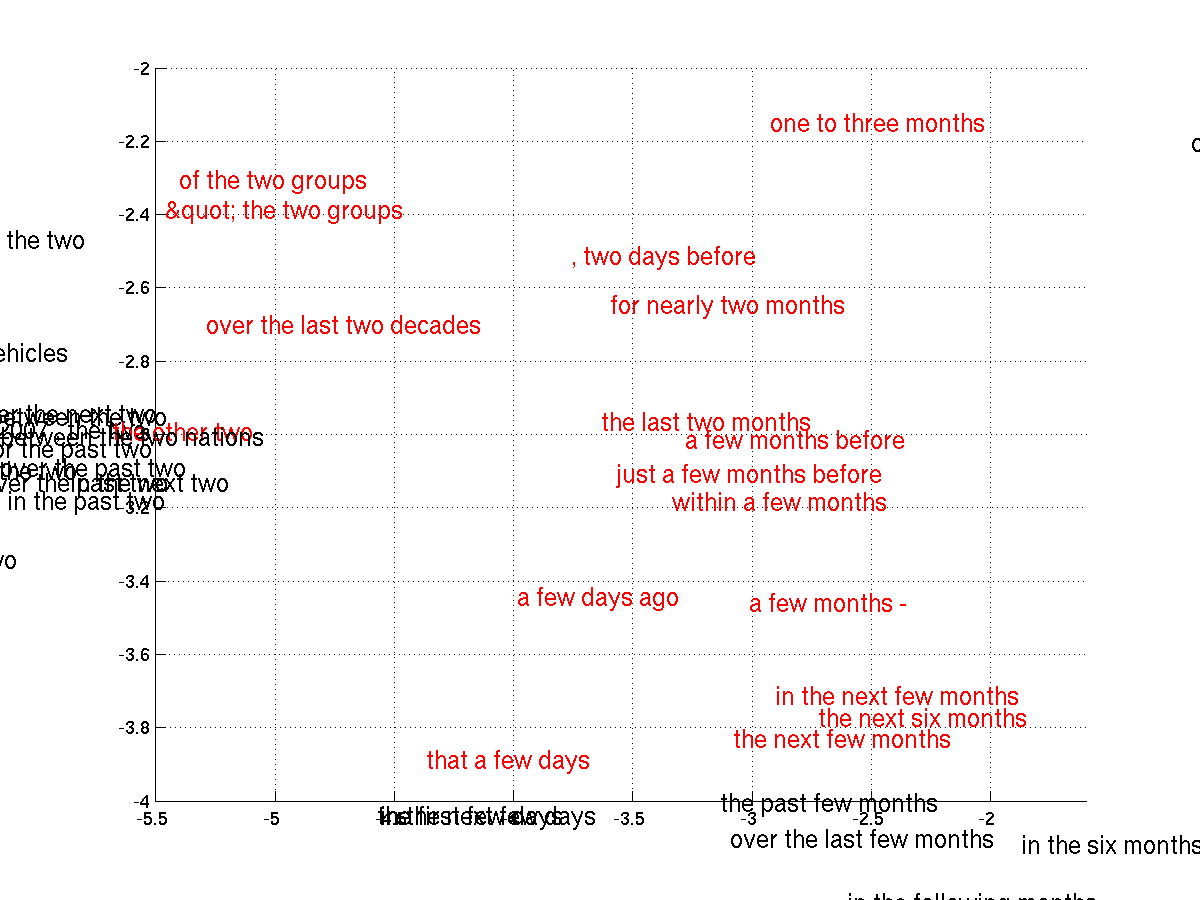
\includegraphics[width=0.99\textwidth]{phrase_zoom2.png}
    \end{minipage}
    \begin{minipage}{0.75\textwidth}
        \centering
        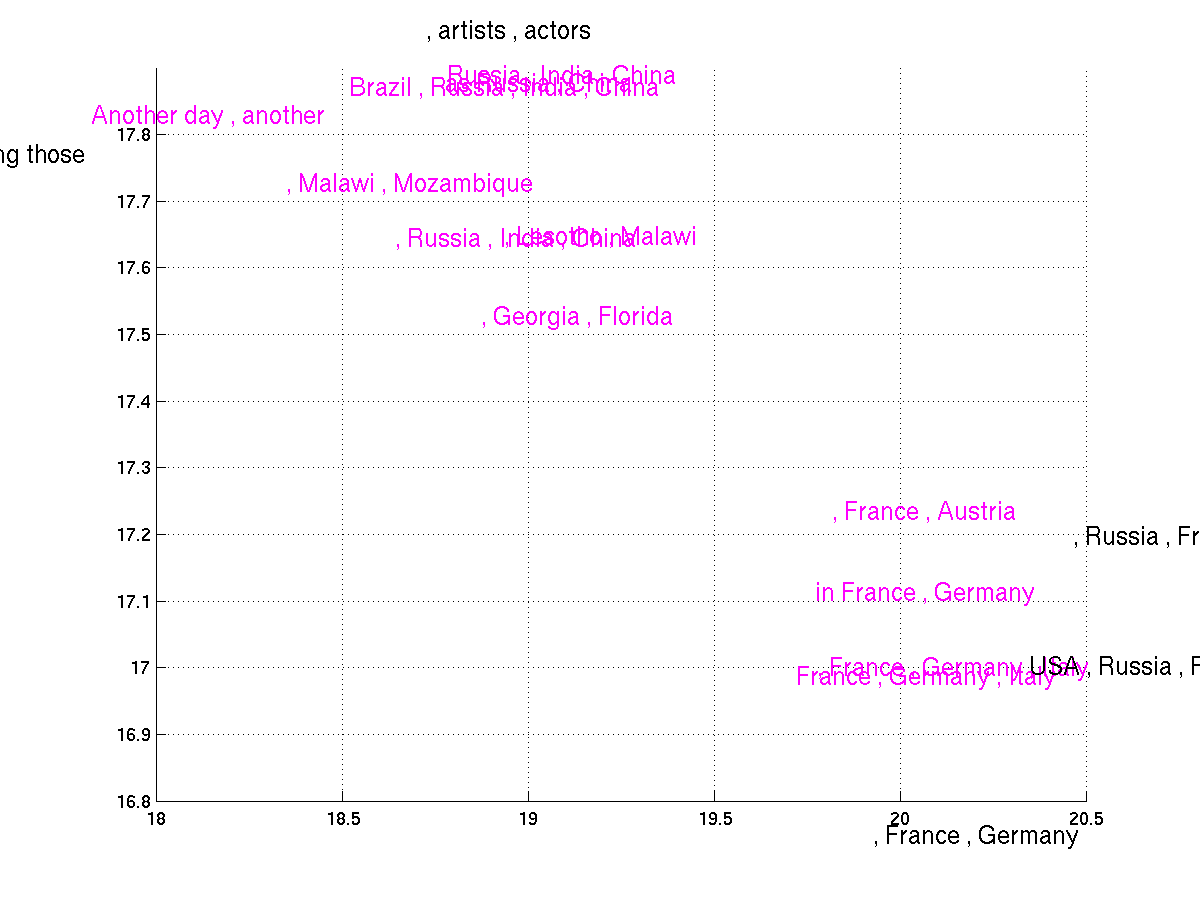
\includegraphics[width=0.99\textwidth]{phrase_zoom3.png}
    \end{minipage}
    \caption{2--D embedding of the learned phrase representation. The top left
    one shows the full representation space (1000 randomly selected points),
while the other three figures show the zoomed-in view of specific regions
(color--coded).} 
\end{figure*}
\end{landscape}

